%%%%%%%%%%%%%%%%%%%%%%%%%%%%%%%%%%%%%%%%%
% Article EcoFoG
% Version 2.1 (23/10/2017)
%
% adapté de :
% Stylish Article
% LaTeX Template
% Version 1.0 (31/1/13)
%
% This template has been downloaded from:
% http://www.LaTeXTemplates.com
%
% Original author:
% Mathias Legrand (legrand.mathias@gmail.com)
%
% License:
% CC BY-NC-SA 3.0 (http://creativecommons.org/licenses/by-nc-sa/3.0/)
%
%%%%%%%%%%%%%%%%%%%%%%%%%%%%%%%%%%%%%%%%%


%----------------------------------------------------------------------------------------
%	PACKAGES AND OTHER DOCUMENT CONFIGURATIONS
%----------------------------------------------------------------------------------------

\documentclass[fleqn,10pt]{ArtEcoFoG} % Document font size and equations flushed left

\setcounter{tocdepth}{3} % Show only three levels in the table of contents section: sections, subsections and subsubsections


% Pandoc environments
\usepackage{framed}
\usepackage{fancyvrb}
\providecommand{\tightlist}{%
  \setlength{\itemsep}{0pt}\setlength{\parskip}{0pt}}
\newcommand{\VerbBar}{|}
\newcommand{\VERB}{\Verb[commandchars=\\\{\}]}
\DefineVerbatimEnvironment{Highlighting}{Verbatim}{commandchars=\\\{\}, fontsize=\scriptsize} % Code R
\definecolor{shadecolor}{RGB}{248,248,248}
\newenvironment{Shaded}{\begin{snugshade}}{\end{snugshade}}
\newcommand{\KeywordTok}[1]{\textcolor[rgb]{0.13,0.29,0.53}{\textbf{{#1}}}}
\newcommand{\DataTypeTok}[1]{\textcolor[rgb]{0.13,0.29,0.53}{{#1}}}
\newcommand{\DecValTok}[1]{\textcolor[rgb]{0.00,0.00,0.81}{{#1}}}
\newcommand{\BaseNTok}[1]{\textcolor[rgb]{0.00,0.00,0.81}{{#1}}}
\newcommand{\FloatTok}[1]{\textcolor[rgb]{0.00,0.00,0.81}{{#1}}}
\newcommand{\ConstantTok}[1]{\textcolor[rgb]{0.00,0.00,0.00}{{#1}}}
\newcommand{\CharTok}[1]{\textcolor[rgb]{0.31,0.60,0.02}{{#1}}}
\newcommand{\SpecialCharTok}[1]{\textcolor[rgb]{0.00,0.00,0.00}{{#1}}}
\newcommand{\StringTok}[1]{\textcolor[rgb]{0.31,0.60,0.02}{{#1}}}
\newcommand{\VerbatimStringTok}[1]{\textcolor[rgb]{0.31,0.60,0.02}{{#1}}}
\newcommand{\SpecialStringTok}[1]{\textcolor[rgb]{0.31,0.60,0.02}{{#1}}}
\newcommand{\ImportTok}[1]{{#1}}
\newcommand{\CommentTok}[1]{\textcolor[rgb]{0.56,0.35,0.01}{\textit{{#1}}}}
\newcommand{\DocumentationTok}[1]{\textcolor[rgb]{0.56,0.35,0.01}{\textbf{\textit{{#1}}}}}
\newcommand{\AnnotationTok}[1]{\textcolor[rgb]{0.56,0.35,0.01}{\textbf{\textit{{#1}}}}}
\newcommand{\CommentVarTok}[1]{\textcolor[rgb]{0.56,0.35,0.01}{\textbf{\textit{{#1}}}}}
\newcommand{\OtherTok}[1]{\textcolor[rgb]{0.56,0.35,0.01}{{#1}}}
\newcommand{\FunctionTok}[1]{\textcolor[rgb]{0.00,0.00,0.00}{{#1}}}
\newcommand{\VariableTok}[1]{\textcolor[rgb]{0.00,0.00,0.00}{{#1}}}
\newcommand{\ControlFlowTok}[1]{\textcolor[rgb]{0.13,0.29,0.53}{\textbf{{#1}}}}
\newcommand{\OperatorTok}[1]{\textcolor[rgb]{0.81,0.36,0.00}{\textbf{{#1}}}}
\newcommand{\BuiltInTok}[1]{{#1}}
\newcommand{\ExtensionTok}[1]{{#1}}
\newcommand{\PreprocessorTok}[1]{\textcolor[rgb]{0.56,0.35,0.01}{\textit{{#1}}}}
\newcommand{\AttributeTok}[1]{\textcolor[rgb]{0.77,0.63,0.00}{{#1}}}
\newcommand{\RegionMarkerTok}[1]{{#1}}
\newcommand{\InformationTok}[1]{\textcolor[rgb]{0.56,0.35,0.01}{\textbf{\textit{{#1}}}}}
\newcommand{\WarningTok}[1]{\textcolor[rgb]{0.56,0.35,0.01}{\textbf{\textit{{#1}}}}}
\newcommand{\AlertTok}[1]{\textcolor[rgb]{0.94,0.16,0.16}{{#1}}}
\newcommand{\ErrorTok}[1]{\textcolor[rgb]{0.64,0.00,0.00}{\textbf{{#1}}}}
\newcommand{\NormalTok}[1]{{#1}}
\usepackage{longtable,booktabs}
\usepackage{caption}
% These lines are needed to make table captions work with longtable:
\makeatletter
\def\fnum@table{\tablename~\thetable}
\makeatother
% longtable 2 columns
% https://tex.stackexchange.com/questions/161431/how-to-solve-longtable-is-not-in-1-column-mode-error
\makeatletter
\let\oldlt\longtable
\let\endoldlt\endlongtable
\def\longtable{\@ifnextchar[\longtable@i \longtable@ii}
\def\longtable@i[#1]{\begin{figure}[t]
\onecolumn
\begin{minipage}{0.5\textwidth}\scriptsize
\oldlt[#1]
}
\def\longtable@ii{\begin{figure}[t]
\onecolumn
\begin{minipage}{0.5\textwidth}\scriptsize
\oldlt
}
\def\endlongtable{\endoldlt
\end{minipage}
\twocolumn
\end{figure}}
\makeatother

\usepackage{graphicx,grffile}
\makeatletter
\def\maxwidth{\ifdim\Gin@nat@width>\linewidth\linewidth\else\Gin@nat@width\fi}
\def\maxheight{\ifdim\Gin@nat@height>\textheight0.8\textheight\else\Gin@nat@height\fi}
\makeatother
% Scale images if necessary, so that they will not overflow the page
% margins by default, and it is still possible to overwrite the defaults
% using explicit options in \includegraphics[width, height, ...]{}
\setkeys{Gin}{width=\maxwidth,height=\maxheight,keepaspectratio}

% User-adder preamble
\usepackage{textcomp} \DeclareUnicodeCharacter{B0}{\textdegree}
\hyphenation{sa-plings} \usepackage{longtable,tabu}

%----------------------------------------------------------------------------------------
%	ARTICLE INFORMATION
%----------------------------------------------------------------------------------------

\JournalInfo{\ }
\Archive{\ }

\PaperTitle{Inescapable Taxonomists: Workable Biodiversity Management Based on a
Minimum Field Work} % Article title

\Authors{
Ariane Mirabel\textsuperscript{1*}\\ Eric Marcon\textsuperscript{1}\\ Bruno Hérault\textsuperscript{2}
} % Authors
\affiliation{
\textsuperscript{1}UMR EcoFoG, AgroParistech, CNRS, Cirad, INRA, Université des Antilles,
Université de Guyane.\\ \hspace{1em} Campus Agronomique, 97310 Kourou, France.\\\textsuperscript{2}INPHB (Institut National Ploytechnique Félix Houphoüet Boigny)\\ \hspace{1em} Yamoussoukro, Ivory Coast
}
\affiliation{*\textbf{Corresponding author}: ariane.mirabel@ecofog.gf, https://github.com/ArianeMirabel} % Corresponding author

\Keywords{Biodiversity Measurement, Tree Community, Neotropical Forests, Botanical Uncertainty Propagation, Bayesian Estimator} % Keywords - if you don't want any simply remove all the text between the curly brackets
\newcommand{\keywordname}{Keywords} % Defines the keywords heading name

%----------------------------------------------------------------------------------------
%	ABSTRACT
%----------------------------------------------------------------------------------------

\Abstract{
Assess the fate of Neotropical forests requires to accurately measures
are the base of reliable foret monitoring, crucial to assess the fate of
neotropical forests in the current changing climate. The costs of
botanical inventories and the taxonomic complexity of Neotropical
forests make predominant forest inventories in vernacular names,
although these hold high botanical uncertainty. Several methods proposed
to compensate botanical uncertainties but none allowed reliable neither
functional nor fine-scale diversity approaches. Here we offer a
polyvalent diversity estimator propagating botanical uncertainties and
workable in numerous specific cases. From a large neotropical
inventory,we calibrated the stimator and through simulations we
determined an ideal inventory protocol optimizing the costs and the
accuracy of forest inventories. Our study first highlighted the
unavoidable use to real inventories, compared to general
vernacular/botanical tables, and the inescapable recourse to taxonomists
to ensure robust diversity survey. Then our simulations allowed
estimated the minimum sampling size (XX trees) and percentage of species
accurately identified (80\% of species known) for inventories to allow
diversity estimations with a 10\% error. The diversity estimator
effectively assessed diversity for a variety of pre-logging and
experimental forest monitoring, acknowledging the rescourse to
taxonomists, and enabled to design optimized inventory protocols.
}

%----------------------------------------------------------------------------------------

\begin{document}

\selectlanguage{english}

\flushbottom % Makes all text pages the same height

\maketitle % Print the title and abstract box

\tableofcontents % Print the contents section

\thispagestyle{empty} % Removes page numbering from the first page

%----------------------------------------------------------------------------------------
%	ARTICLE CONTENTS
%----------------------------------------------------------------------------------------


\section{Introduction}\label{introduction}

The variety of tree species, their assemblages in space and their
dynamics in time are determinant of forests productivity and functioning
\citep{Magurran1988, Cardinale2012}. Preserve tree diversity is crucial
to maintain forests functioning and services, specifically in
hyper-diverse tropical forests where the biodiversity is as threatened
as it is valuable and unexplored \citep{Koh2010, Barlow2018}. Handling
the conservation and management of tree diversity requires setting
sensitive protection areas and sustainable forest management calibrated
according to their spatial and temporal patterns and determinants
\citep{Margules2000, Purvis2000, Gibson2011a, FAO2009, Sist2015}.

Correctly measure, map and manage forests biodiversity require accurate
and large forest monitoring. The precision of forest inventories,
though, is often limited by their significant cost in terms of time,
money, and logistic \citep{Feeley2011}. Sampling methods were optimized
to minimize these costs and maximize inventory accuracy. Some approaches
would restrict inventories to some DBH or height classes, to specific
taxa, or would opt for inventories at family or genus level. These
methods efficiently translated biodiversity patterns at regional scales
and along wide ecological gradients
\citep{Steege2000, Higgins2004, Rejou-Mechain2011, Pos2014}. However,
these methods were either limited to small areas (under 1ha), sometimes
remained biased or holding significant uncertainty, and usually proved
limited to detect subtle diversity aspects and to desentangle richness
from equitability parameters
\citetext{\citealp{Phillips2003a}; \citealp{Valencia2013}; \citealp[
]{Guitet2014b}; \citealp{Vellend2008}; \citealp{Prance1994}}. Another
approach proposed to use inventories in vernacular names instead of
botanical species. Vernacular names indeed are easier to attribute, more
common and usually do not require vouchers collection or posterior
botanical identification. Similarly though, vernacular names entail
significant botanical uncertainties as the association with botanical
species is usually highly variable in space and time
\citep{Oldeman1968}. Besides, rough vernacular inventories would not
suit the needs of functional and phylogenetic approaches that require
identification at the botanical species to comply with phylogenetic and
functional database. However the approach through vernacular names
deserves further attention. First, it gives the opportunity to analyze
pre-logging inventories conducted in large areas by logging companies.
Second, as exhaustive inventories, they allow some post-process based on
vernacular/botanical names association and allow the building of
reliable diversity estimators
\citep{TerSteege2006, Feldpausch2006, Rejou-Mechain2008, Rejou-Mechain2011}.
Following this idea \citet{Guitet2014b} proposed a framework propagating
vernacular names taxonomic uncertainties in diversity measures. The
propagation framework was based on Monte-Carlo processes estimating
forest diversity from the vernacular-botanical name association. These
association combined prior information from both general taxa-abundance
correspondence table \citep{De2009} and reference field inventories. The
framework successfully rendered the ranking of plots diversity, but
remained restricted to large environmental gradient and for highly
different communities \citep{Guitet2014b, Guitet2013}. In this study we
offer to refine this framework and adapt it to diversity estimation at
smaller spatial scales. The following diversity estimator is based on
the specific case of the studied community and the inventory protocol.
The diversity estimator besides suits all inventories whatever the ratio
of botanical determination, \emph{i.e.} ratio of vernacular compared to
botanical names. It besides suits experimental specific as well as
pre-logging inventories where only the commercial or most recognizable
species are identified at species level.

Such diversity estimator allows maximizing the accuracy of diversity
measures while minimizing the sampling effort, \emph{i.e.} the size of
inventoried communities and the number of accurately identified species.
In this perspective we thought to calibrate an ideal inventory protocol
optimized in terms of sampling effort and determination degree. From a
real inventory, with complete vernacular and botanical identifications,
we simulated ranges of sampling efforts and identification degrees along
which we examined the bias and variability of the diversity estimator.

In this study we \emph{(i)} redesigned a diversity estimator based on a
Bayesian framework accounting for both general taxa-association tables
and specific field inventories, and \emph{(ii)} applied the estimator to
a real Neotropical forest inventory to determine the sampling effort and
determination degree of an ideal inventory protocol.

\section{Methods}\label{methods}

\subsection{Study community}\label{study-community}

We based our analyses on the inventory of a Neotropical rainforest, from
the Paracou Research Station in French Guiana (5°18'N and 52°53'W). The
experimental site stands in a lowland tropical rainforest with a flora
dominated by \emph{Fabaceae}, \emph{Chrysobalanaceae},
\emph{Lecythidaceae} and \emph{Sapotaceae} families. Mean mean annual
temperature is 26°C. and the mean annual precipitations average
\(2980 mm.y^-1\) (30-y period) with a 3-months dry season
(\(< 100 mm.months-1\)) from mid-August to mid-November and a one-month
dry season in March \citep{Wagner2011}. Elevation ranges between 5 and
50 m and soils correspond to thin acrisols over a layer of transformed
saprolite with low permeability, generating lateral drainage during
heavy rains \citep{IUSSWorkingGroupWRB2015}. We used the 2015 inventory
of six permanent plots of undisturbed forest (6.25ha each, 37.5ha
inventoried in total). During inventories trees are identified first
with a vernacular name assigned by the forest worker team, and afterward
with a scientific name assigned by botanists during regular botanical
campaigns. The community inventoried ancompasses 22 904 trees belonging
to 375 species and 63 families, identified by 290 different vernacular
names. The initial taxonomic uncertainty was 3\% of the community,
\emph{i.e.} the proportion of trees not identified with a botanical
name.

\subsection{Diversity measures}\label{diversity-measures}

Among the large panel of diversity indices we examined here the family
of q-generalized (Tsallis) entropy, widely adopted to assess all aspects
of taxonomic, functional and phylogenetic diversities. The Tsallis
diversity indices derive from a general formula, modulated by an order q
emphasizing species frequency \eqref{eq:TsallisEntropy}.

\begin{equation}
^qD = \sum_{i=1}^{N}{\left( p_i^q \right)^{\frac{1}{1-q}} }
\label{eq:TsallisEntropy}
\end{equation}

In the diversity formula, species relative abundance \(p_i\) in a
community of \(N\) species is raised at the power \(q\) that is the
order of the diversity. The higher the order \(q\), the higher the
emphasis on common vs.~rare species, so browsing a range of order \(q\)
corresponds assess a gradient balance between richness and evenness. The
formula retrieves species richness for \(q = 0\) , Shannon diversity for
\(q = 1\) where richness and evenness are equally accounted for and
Simpson diversity, that can be undestood as the diversity of common
species, for \(q = 2\). The Tsallis diversity indices would eventually
be converted into equivalent number of species in our framework. The
conversion in equivalent number of species, through Hill transformation,
allows understandable analysis and comparisons among communities
\citep{Hill1973, Keylock2005, Jost2006}.

\subsection{Diversity estimator}\label{diversity-estimator}

The estimation framework is based on the distribution of the diversity
of theoretical, fully determined communities. For each incomplete
inventory, 1 000 theoretical inventories are simulated through the
replacement by a Monte-Carlo scheme of vernacular names by botanical
ones.

Theoretical inventories are simulated from the association probability
between vernacular names and the \(N\) botanical names inventoried. This
association is modelled for each vernacular name by a multinomial
distribution on the \(s_N\) botanical species
\(M([s_1, s_2, …, s_N] ,[\alpha_1, \alpha_2,…, \alpha_N])\), where
\([s_1, s_2, …, s_N]\) are the species recorded in the inventory and
\([\alpha_1, \alpha_2,…, \alpha_N]\) their association probability with
the vernacular name.

The probabilities \([\alpha_v]\) were determined with a Bayesian
framework based on the combination of botanical expertise and
real,complete inventories. First, the estimation of \([\alpha_v]\) was
based on prior information from experts' knowledge in the form of a
taxa-association table listing all botanical names likely corresponding
to the vernacular name \(v\). For a vernacular name \(v\) a vector
\([\lambda_v]\) giving the association probability
\(\lambda_i={}^1/m_v\) for \(v\) to be associated with the botanical
name \(i\). When no association between \(v\) and \(i\) was established,
\(\lambda_i={}^\epsilon\big/_{N-n_{table}}\), with \(\epsilon\) standing
for a background noise set to 0.01 here. Second, the estimation of
\([\alpha_v]\) was based on reference field inventory giving the
observed vernacular/botanical association frequency \(\phi_i\)
constituting the vector \([\phi_v]\). Similarly, a background noise
\(\epsilon=0.01\) was attributed to botanical names with no observed
association with \(v\), giving the association probability
\(\lambda_i={}^\epsilon\big/_{N-n_{field}}\). The two vectors
\(\lambda^v\) and \(\phi^v\) were combined in a Multinomial-Dirichlet
scheme \citep{McCarthy2007} to model the final \([\alpha_v]\)
distribution.

The relevance of the two parameters was tested in weighting their
importance in the formula. With \(w\) the wieghting parameter,assuming a
distribution of \([\phi_i]^v\) conditionally to \([\alpha_i]^v\) we had
\eqref{eq:weighting}

\begin{equation}
[\alpha_i^v]: 
\Big[\alpha_i^v | _{(1-w)\lambda_i^v ,w.\phi_i^v}\Big] =Dirichlet\Big((1-w)\phi_i^v+w.\lambda_i^v\Big)
\label{eq:weighting}
\end{equation}

When \(w=0\) only the reference field inventory was considered, when
\(w=0.5\) both dataset weighted equally and when \(w=1\) only the
general taxa-association table was considered.

\subsection{Simulation of the uncertainty gradient and determination of
optimal framework and reference
protocol}\label{simulation-of-the-uncertainty-gradient-and-determination-of-optimal-framework-and-reference-protocol}

To determine the impact of the determination ratio
\[\big(\cfrac{\text{number of vernacular name}}{\text{number of trees}}\big),\]
we simulated gradient of determination ratio by removing the botanical
identification of an increasing proportion of species in inventory of
reference. In the initial inventory a Kendall test
(\(\tau = -0.46, p < 10^-16\)) showed that the probability of a species
to be undetermined in an inventory is negatively linked to its
abundance. Therefore, to simulate the indetermination gradient we
sampled the species according to their abundance: the probability
\(p_i\) of species \(i\) to be ``undetermined'' in a simulation was
\(f_i^{-0.1}\), with \(f_i\) its frequency. We applied our framework
along the gradient of indetermination ratio to calibrate the framework
and specifically find the best balance \(w\) between general
taxa-association tables and reference field inventories. We also
determined the minimum sampling effort for the reference field
inventory, in terms of number of trees required to infer a correct
vector of association frequencies \([\phi_v]\). We tested a range of
sampling effort from 500 to 22 000 trees randomly selected from the
whole inventory to calculate \([\phi_v]\). All our simulations of a
gradient of indetermination ratio and sampling effort were repeated 1
000 times. From these iteration we assessed the performance of the
diversity estimators through the average estimation bias, measured as
the difference between the estimation and the diversity of the reference
inventory \citep{Baltanas2009}, and through the relative estimation
error, measured as the 95\% confidence interval. We restricted our
analysis on the Richness, Shannon and Simpson diversities which informs
about both community's richness and equitability. To validate the
convergence of the model we first simulated 100 values and realized a
bootstrap through independent randomized subsamples of 2 to 100
simulations .

\section{Results}\label{results}

\subsection{Impacts of undetermination ratios and ideal
settings}\label{impacts-of-undetermination-ratios-and-ideal-settings}

When considering both general taxa-correspondence table and reference
field inventory diversity estimator showed a positively bias that
increased with the indetermination ratio (Figure
\ref{fig:Fig1}\emph{(a)}). The bias of the estimator was besides
increasing with the order of diversity q. For the order \(q = 0\) the
estimation did not significantly differ from the initial value of the
real inventory while for the order \(q = 1\) the overestimation reached
45\% of the initial diversity and for the order \(q = 2\) the
overestimation reached 57\%. When only the general taxa-correspondence
table is considered (Figure \ref{fig:Fig1}\emph{(b)}) the richness was
highly underestimated, it reached 50\% when the whole inventory was in
vernacular names, while the Shannon and Simpson indices were both
significantly overestimated, their respective bias reaching 67\% and
125\%. When only the reference field inventory is considered (Figure
\ref{fig:Fig1}\emph{(c)}) there were still estimation biases but they
did not exceed 15\% for any order of diversity.

We performed a bootstrap of the 100 simulations that showed a
stabilization of variances after 60 simulations. We therefore set the
number of simulations at 60 in the final script (Figure
\ref{fig:FigS1}).

\begin{figure*}
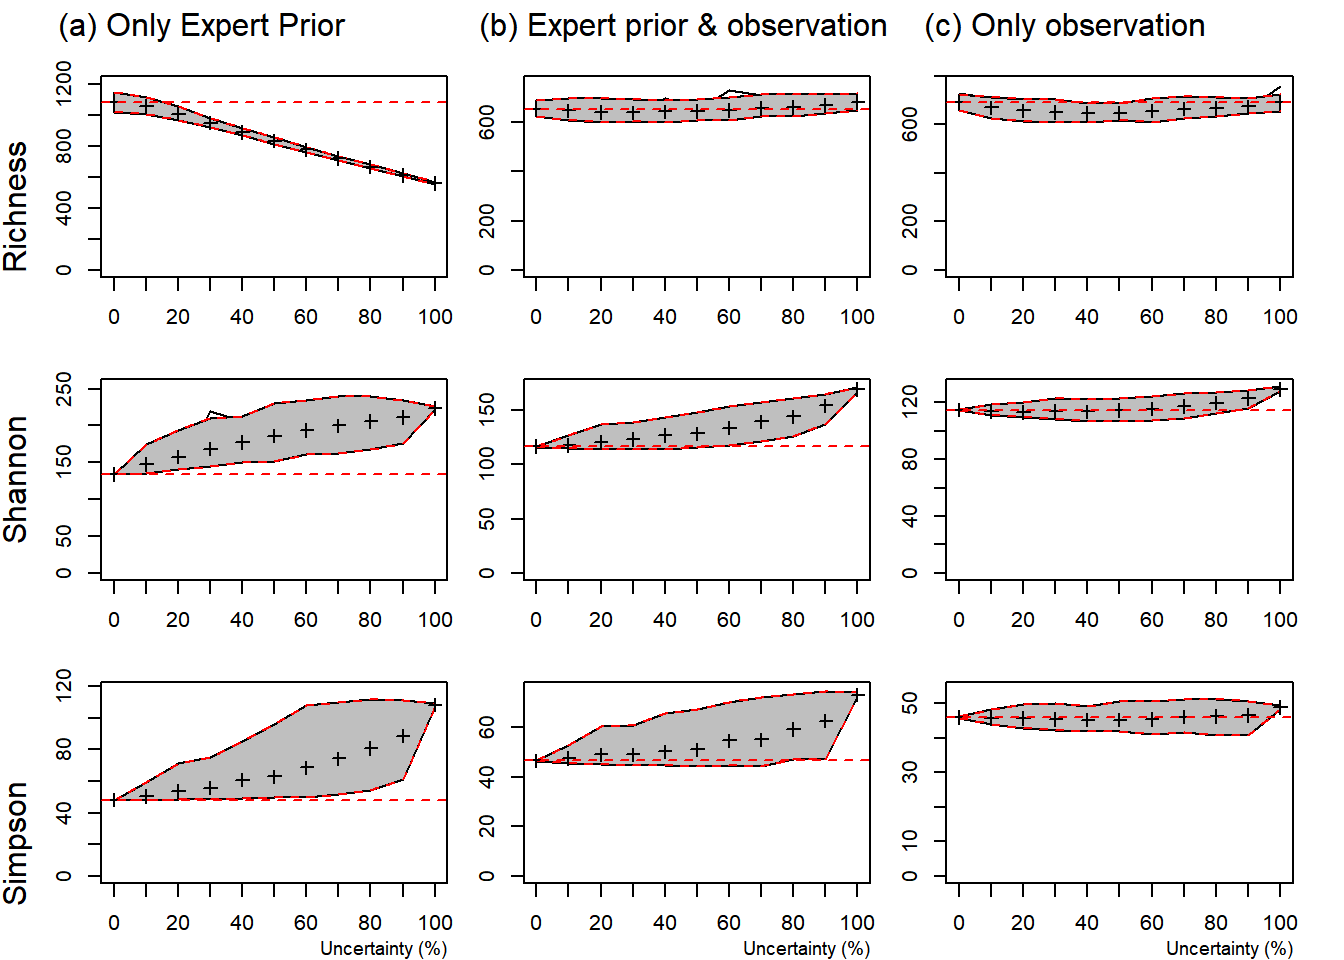
\includegraphics[width=1\linewidth]{TaxonomicUncertainty_files/figure-latex/Fig1-1} \caption{Indices degradation along a taxonomic uncertainty gradient. 95\% envelopes of the Richness, Shannon and Simpson indices calculated through our propagation method along an uncertainty gradient from 0 to 100\% of undetermined species. In (a) Only expert prior is considered to compute the association frequencies, in (b) both expert and observation prior are equally accounted for in the propagation method and in (c) only the observation prior is considered.}\label{fig:Fig1}
\end{figure*}

\begin{quote}
r Fig2, out.width = `60\%', echo=FALSE,fig.cap=``Degradation along a
taxonomic uncertainty gradient of diversity estimated from a reference
field inventories of 2 000 trees. 95\% envelopes of the Richness,
Shannon and Simpson diversities calculated along an uncertainty gradient
from 0 to 100\% of undetermined species.''
\end{quote}

\subsection{Calibrating the sampling
effort}\label{calibrating-the-sampling-effort}

We simulated a gradient of sampling effort for the reference field
inventory, in terms of number of trees required to infer a the vector of
association frequencies \([\phi_v]\), to identify the minimum effort for
reliable diversity estimators. We tested a range of sampling effort from
500 to 22 000 trees randomly selected from the whole inventory (Figure
\ref{fig:Fig3}). The biases of the estimators decreased with the order
of diversity. The richness of reference is not faithfully retrieved
before recovering the whole inventory (Figure \ref{fig:Fig3}\emph{(a)})
but the 95\% confidence interval of the estimator does not exceed 7\% of
the initial diversity. The Shannon and Simpson estimators showed lower
biases, the bias of Shannon estimator falls to 15\% for 2 000 reference
trees (Figure \ref{fig:Fig3}\emph{(b)}) and the bias of Simpson
estimator falls to 6\% (Figure \ref{fig:Fig3}\emph{(c)}).

\begin{figure*}
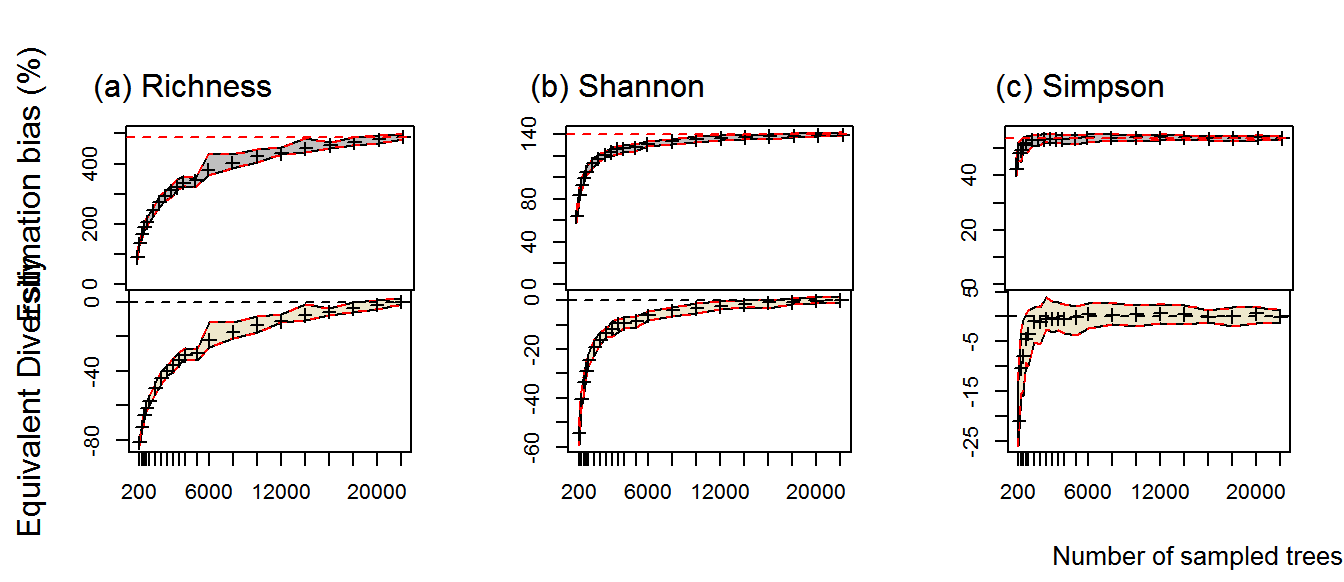
\includegraphics[width=1\linewidth]{TaxonomicUncertainty_files/figure-latex/Fig3-1} \caption{Degradation along a sampling effort gradient of the Richness, Shannon and Simpson diversities estimated for the reference inventory in vernacular names. The propagation method to estimate the diversities is only based on the reference field inventory. Above plots correspond to the estimated diversity in equivalent number of species and below plots correspond to the relative bias of the estimation compared to the value of the reference field inventory. For both dashed lines represent the value of the reference field inventory and crosses and red lines respectively represent the mean, 0.05 and 0.95 quantiles estimated after 1000 iterations.}\label{fig:Fig3}
\end{figure*}

\section{Discussion}\label{discussion}

In this paper we present a method of inventory protocols to correctly
propagate taxonomic uncertainty of vernacular name in the measure of
forest diversity. Our method is based on a Bayesian process which base
is the probability of association between vernacular and botanical
names. The comparison of several methods to build the basic
vernacular-botanical association vectors demonstrated that the biases
and the variability of the diversity estimator were much lower when
reference field inventories are used rather than general
taxa-association table. From this conclusion, we determined the minimum
number of trees for the reference field inventory. To this end we run
the estimation method with a set of association vectors computed from an
increasing number of trees: we found that reference inventories should
be based on a minimum of 2 000 trees, which ensures no more than 10\%
error for Shannon diversity and 1\% error for Simpson diversity. We did
not obtain an unbiased estimator of species Richness but demonstrated a
linear correlation between estimated richness.

\subsection{Prior field inventories for reliable diversity
estimations}\label{prior-field-inventories-for-reliable-diversity-estimations}

We set up a framework providing reliable and accurate diversity
estimations in handling the taxonomic uncertainty of vernacular names
due to their multiple correspondences to botanical species. In the line
of \citet{Guitet2014b} our method propagates the taxonomic uncertainty
to diversity estimators through a Bayesian framework that was either
based on general taxa-correspondence tables or reference field
inventories. We determined the best balance between both dataset in
applying our framework along a gradient of indetermination ratio
\(\big(\cfrac{\text{number of vernacular name}}{\text{number of trees}}\big)\).
Whenever its weight the account of the general taxa-association table
underestimated the Richness and overestimated the Shannon and Simpson
diversities (Figure \ref{fig:Fig1}). The use of general taxa-association
table increases the equitability of the community in inflating the
abundance of rare species at the expense of abundant ones. The
association probabilities computed from this dataset are independent of
species abundance so the vernacular name of a rare species will
indifferently be associated to are or abundant species. The use of a
reference field inventory to the contrary gives vector of association
probability dependent of species abundance and retrieves the real
abundance distribution so the diversity estimator however is much less
biased. A reliable diversity estimator should then be based on reference
field inventory performed beforehand by the working team in the studied
community.

\subsection{Calibration of the reference
inventory}\label{calibration-of-the-reference-inventory}

Reliable diversity estimator should be based on a reference field
inventory ensuring small estimation biases and uncertainty. The
determine the minimum size of this reference inventory we applied our
framework for an gradient of sampling effort, in terms of number of
trees used to compute the association probabilities. We found it
difficult to retrieve the initial richness, as already suggested in
previous analysis comparing random-sampling methods to these based on
restricted inventories \citep{Higgins2004}. However, if the estimator of
richness was biased it varied little and should preserve the ranking of
communities with similar indetermination ratio. This was coherent with
various results linking the whole community richness to that of
communities subsamples \citep{Vellend2008}. The bias of the richness
estimator though is a minor annoyance because for small time and spatial
scale the richness is not necessary the most relevant diversity to
consider \citep{Baraloto2012a, Berry2008a, Cannon1998, Plumptre1996}.
The estimator of Shannon and Simpson diversities were much less biased
and reasonably. Our results showed that from 2 000 trees inventoried
beforehand the Shannon and Simpson estimators respectively had 12\% and
1\% uncertainty.

\section{Conclusion}\label{conclusion}

A keystone for biodiversity conservation is to understand the
determinants of communities assembly, especially in tropical forest
where stands are as complex and species-rich as they are valuable and
uncharted \citep{Magurran1988, Prance1994, Cardinale2012, Sist2015}.
Despite the study of tropical forests structure and composition however
still a need large and intensive sampling in space and time which is
hampered by the important costs of inventories in tropical forests
\citep{Valencia2013}. It is then urgent to develop methods alleviating
the cost of inventories while producing accurate and unbiased estimation
of the diversity. In that respect using vernacular names is promising
because they are easier to attribute, known by the main part of field
workers and proved to bear valuable information. Their reliability at
genus level proved high but variable across tropical regions: it was
estimated around 60-70\% in French Guyana \citep{Hawes2012, Guitet2014b}
and from 32\% to 67\% in Central African \citep{Rejou-Mechain2011}.
Although vernacular names can be used to estimate communities' diversity
they generate significant taxonomic uncertainty due to the multiple
correspondences between botanical and vernacular names. Reliably measure
forest diversity from vernacular names requires setting adapted
protocols and a propagation method of the taxonomic uncertainty. In this
paper we present a method to propagate the taxonomic uncertainty of
vernacular names to the measure of tropical forest diversity. We
calibrated the corresponding inventory protocols to ensure accurate
estimation: at the cost of an initial reference botanical inventory of 2
000 trees Shannon and Simpson diversities are estimated with
respectively 10\% and 1\% accuracy. Our methods is besides workable to
estimate functional and phylogenetic diversities indifferently. The
method is based on reference field inventory and integrates the
specificity of the working team and local forest structure. It is
workable in all contexts and we propose that it be largely applied to
get insights into the issue of vernacular names handling.

%----------------------------------------------------------------------------------------
%	REFERENCE LIST
%----------------------------------------------------------------------------------------

\bibliographystyle{mee}
\makeatletter
% The filename has .bib extension the must be eliminated
\filename@parse{references.bib}
% parse stores the file name in base. Extension starts at the first dot, so don't use dots in file names.
\bibliography{\filename@base}
\makeatother


%----------------------------------------------------------------------------------------

\end{document}
